\documentclass[a4paper, 12pt]{report}

\usepackage{comment}
\usepackage{hyperref}
\usepackage{geometry}
\usepackage{listings}
\usepackage{xcolor}
\usepackage{amsmath}
\usepackage{array}
\usepackage{graphicx}

\geometry{portrait, margin= 0.43in}

\def\tabsize{1.9cm}
\def\ltabsize{1.4cm}

\definecolor{codegreen}{rgb}{0,0.6,0}
\definecolor{codegray}{rgb}{0.5,0.5,0.5}
\definecolor{codepurple}{rgb}{0.58,0,0.82}
\definecolor{backcolour}{rgb}{0.95,0.95,0.92}

\lstset{
	columns=fullflexible,
	frame=single,
	breaklines=true,
	backgroundcolor=\color{backcolour},   
	commentstyle=\color{codegreen},
	keywordstyle=\color{magenta},
	numberstyle=\tiny\color{codegray},
	stringstyle=\color{codepurple},
	basicstyle=\ttfamily\footnotesize,
	keepspaces=true,                 
	numbersep=5pt,                  
	tabsize=2
}


\begin{document}

\title{Arch Linux Tutorial}
\author{Ginger Gengar}
\date{$12^{th}$ July 2022}
\maketitle
\newpage

\tableofcontents
\newpage

\begin{center}
\section{Rationale}
\begin{comment}
\end{comment}
Below explains why this tutorial exists. This tutorial is only valid for Arch Linux that was personally configured. 
%Seperator
%Seperator
%Seperator
%Seperator
\subsection{Why Use a Computer?}
\begin{comment}
\end{comment}
%Seperator
I cannot certainly speak for all users, I use a computer to help me do abstract work. Mathematics is the backbone of most major engineering fields. A lot of things in mathematics can be solved using analytical hand-written solutions, but many real-life problems cannot be solved that way. They must be solved numerically, by manual iteration. This is fine if your problem is small, but once your problem gets large enough, it becomes impossible to do by hand and instead, you have to turn to computers. 
%Seperator
\\~\\What kind of mathematical problems am I referring to? I am referring to ordinary differential equations, large matrix equations, tensor operation and even experimental symbollic computation. Why are these problems important? Solving these mathematical problems allows us to construct bridges, skyscrapers, train networks, cars, ships, aircrafts, rocketry, and most modern technologies we have today. Technology's backbone is theoretical engineering and theoretical engineering's backbone is mathematics, and mathematics can then be solved using general-purpose computers. So computers in this regard represent the last step of computing answers to. Computers are NOT A SUBSTITUTE for HUMAN THOUGHT.
%Seperator
\\~\\What other things can be done by tinkering with a computer? Automation of manufacturing, moving actuators, flying aircrafts and driving cars. Lower level electronics that can marginally be called computers also perform alot of vital tasks in multiple industries, though I am not an expert in this regard, I deal more with the theoretical computations so far. There are many other applications of computer beyond what I have discussed, but the above are already very good reasons to learn computing.

%Seperator
%Seperator
%Seperator
%Seperator
\subsection{Why Use Linux?}
\begin{comment}
\end{comment}
%Seperator
One of the most astounding things I still remember to this day switching from Windows to Linux (Ubuntu) was the existence of package managers. For some reason my machine did not come with mingw, which made it incapable of compiling \texttt{C}. I spent almost 2 days trying to install mingw navigating through old sites, and being concerned of accidentally installing malware. Eventually I failed to install mingw. In Linux (Ubuntu) though, the \texttt{C} compiler \texttt{gcc} was pre-installed, and even if it wasn't, a simple command to the package manager solves all of 2 days worth of problems in just 2 minutes, not even.
%Seperator
\\~\\I also attempted to install a linear algebra library called \texttt{armadillo}. I also wanted to try out another linear algebra library \texttt{eigen}. I had to go through so many hoops installing all of the dependencies manually for \texttt{armadillo} such as \texttt{BLAS}, \texttt{SuperLU}, and others. With a linux system, a simple package manager command installs everything perfectly. So the point is, the package manager in Linux is absolutely necessary for any real programming work and is one of many great reasons to use Linux.
%Seperator
\\~\\It didn't mean much when I first started Linux, but Linux is largely customizable. The text editor, kernel version, window manager, compositor, shell, and many other utilities can be configured and customized to the user's liking. This makes the Linux operating system an incredibly personal and efficient machine. Think about the Linux operating system as a lego piece whose parts can be defined by the user themselves and chosen. This also means that no 2 Linux operating system are exactly alike because each user has their own configurations and choice of programs. 
%Seperator
\\~\\The customizability of Linux also permits a variety of workflows, including \texttt{cli}-based workflows. \texttt{cli} stands for command line interface. This is a way to use the computer that abandons the mouse altogether and does everything from just the keyboard. It is faster and easier to do many tasks that way. In this tutorial, \texttt{cli} would be used extensively.
%Seperator
The last reason I have is an ideological one, which is that the Linux operating system is part of a free operating system. Free here as define by the \texttt{GNU} does not necessarily mean free of cost (although Linux is free of cost) but instead, free here means the users are free to examine the system in great detail, learn and expand it on their own. This is important because it gives the users the reigns to how computing is done. Users can verify no malware is pre-installed on the machine, and that the computer performs up to user expectations. Users are also not dependent on corporates which is good.

%Seperator
%Seperator
%Seperator
%Seperator
\subsection{Why Arch Linux?}
\begin{comment}
\end{comment}
%Seperator
A Linux distribution just means a version of Linux. Arch Linux is a Linux distribution, which means that Arch Linux is a version of the Linux operating system. To be clear, all Arch Linux systems are part of the Linux family, but not all Linux systems is Arch Linux. There are a few reasons why Arch Linux is a good Linux operating system:
%Seperator
\\~\\Arch Linux supports both binary installs and building from source. Compiled programs are translated from ther text form into machine code, which are 1's and 0's in human-unreadable form. The act of translating text format into machine code is called compilation. Binary installation is downloading those raw machine code and putting them in the appropriate directory inside the system. Building from source or source installation is downloading the human-readable text form, and then performing the compilation process on the user's machine before installing the resulting binary in the user's machine. Building from source always takes longer than binary install, but has the potential of resulting in a higher performing installed program.  Arch Linux supports both types of installs, which makes it very flexible and can install a very large variety of programs.
%Seperator
\\~\\Arch Linux is also very minimal. Minimal means that the base Arch Linux system has very few things installed in it. This means that users are free to build the system from the ground up, specifying the browser, terminal, window manager, compositor, status bar, text editor and other details themselves. A minimal system IS NOT IDEAL for users who believe an operating system should work out of the box. In a minimal system, one has to specify everything themselves, which is where the customization power of Linux is best revealed. 
%Seperator
Users who want to trade customization power for convenience should just try another distribution like Ubuntu, Linux Mint, Manjaro, etc. A non-minimal system has drawbacks when the user attempts to customize it because then the user has to uninstall unnecessary pre-installed packages, and then figure out the relationship between different packages and how to break their link and so on, which is more complicated than just configuring the system on your own. By configuring the system on your own, at least the user knows the different relationship bewteen different softwares they themselves have installed.

%Seperator
%Seperator
%Seperator
%Seperator
%Seperator
\section{Program Configurations}
\begin{comment}
\end{comment}
In this section, we will learn how to configure basic programs. 

%Seperator
%Seperator
%Seperator
%Seperator
\subsection{Basic Terminal Usage}
\begin{comment}
\end{comment}
Starting programs, writing, and almost anything can be done through the terminal. To open a new terminal press:
\begin{lstlisting}
super + enter
\end{lstlisting}
The super key is the command key, or the windows key on a typical keyboard. A new terminal instance should appear on pressing the keybinding above. To quit the terminal instances, press:
\begin{lstlisting}
ctrl + shift + w
\end{lstlisting}
These keybindings have not been changed from the default in kitty. Kitty has tabs and windows. Windows are inside a tab. To open a new tab, press:
\begin{lstlisting}
ctrl + shift + t
\end{lstlisting}
To navigate to the tab on the left
\begin{lstlisting}
ctrl + shift + left
\end{lstlisting}
To navigate to the tab on the right:
\begin{lstlisting}
ctrl + shift + right
\end{lstlisting}
Within a single tab, it is possible to open multiple windows. To do this, press:
\begin{lstlisting}
ctrl + shift + enter
\end{lstlisting}
To navigate to the left window,
\begin{lstlisting}
ctrl + shift + [
\end{lstlisting}
To navigate to the right window,
\begin{lstlisting}
ctrl + shift + ]
\end{lstlisting}
The keybinding \texttt{ctrl + shift + w} can close windows one at a time and tabs as well, try experimenting with it. To open a new tab between existing tabs, press:
\begin{lstlisting}
ctrl + t
\end{lstlisting}
This should cover the basics of terminal navigation.

%Seperator
%Seperator
%Seperator
%Seperator
\subsection{Basic Window Manager Usage}
\begin{comment}
\end{comment}
Without anything else open, user resides in the first workspace. To go to the second workspace, press:
\begin{lstlisting}
super + 2
\end{lstlisting}
To go the third workspace,
\begin{lstlisting}
super + 3
\end{lstlisting}
Entering a different number will go to that workspace.  To go back to the original workspace, press:
\begin{lstlisting}
super + 1
\end{lstlisting}
Try opening 2 terminals by pressing \texttt{super + enter} twice for the two terminals. Try opening multiple tabs on one of them by pressing \texttt{ctrl + shift + t} successively for one of the terminals. To navigate between the terminal instances press:
\begin{lstlisting}
super + left
\end{lstlisting}
Alternatively, one can press:
\begin{lstlisting}
super + right
\end{lstlisting}
To make the terminal instances tile differently, One can navigate to either one of the terminal instances and press:
\begin{lstlisting}
super + shift + left
\end{lstlisting}
One can experiment with the following commands for different ways to tile the terminals:
\begin{lstlisting}
super + shift + up
super + shift + down
super + shift + right
\end{lstlisting}
One can think of the \texttt{super + shift} as the keybinding to "hold and drag" a particular terminal instance. The same logic can be applied to put terminal instances and other programs in different windows. Try navigating to one of the terminal instances and then pressing:
\begin{lstlisting}
super + shift + 2
\end{lstlisting}
Pressing different numbers will move the terminal instances or other programs to different workspaces. For example, to move a terminal instance to the third workspace, navigate to the terminal instance and press:
\begin{lstlisting}
super + shift + 3
\end{lstlisting}
The window manager also can force quit a window. To kill a particular window, navigate to it and then press:
\begin{lstlisting}
super + shift + q
\end{lstlisting}
This should cover the basics of how the window manager works.

%Seperator
%Seperator
%Seperator
%Seperator
\subsection{Basic Core Utilities}
\begin{comment}
\end{comment}
To make a new file use type in the following command in a terminal instance:
\begin{lstlisting}
touch Pokemon.txt
\end{lstlisting}
\texttt{touch} is one of the core utilities in the Linux system, and the command above just means create the file named \texttt{Pokemon.txt} inside the current directory. Changing \texttt{Pokemon.txt} with another name would change the name of the file you are creating. For example, to create another file named \texttt{Digimon.dat} one can simply just type inside the terminal:
\begin{lstlisting}
touch Digimon.dat
\end{lstlisting}
One difference coming from a \texttt{Windows} operating system is that file name extensions like \texttt{.txt}, \texttt{.dat}, \texttt{.exe} in windows tell the operating system what to do with those files. In Linux, file name extensions are more like suggestions for the content inside. The operating system will not care what the extension of those files are. So in a Linux system, naming a file \texttt{Pokemon.txt} and \texttt{Pokemon.dat} will not change how the computer treats the files. Now to see the list of files and folders in the current directory, invoke the \texttt{list} command by typing in the terminal:
\begin{lstlisting}
ls
\end{lstlisting}
If you do that, then you will see the names of the files we have created in the previous prompts. The way to delete files is to invoke the \texttt{remove} command. To delete the file \texttt{Pokemon.txt} that is in the current directory, type in:
\begin{lstlisting}
rm Pokemon.txt
\end{lstlisting}
The \texttt{rm} command has to be used with great caution. Deleting a file or directory using the \texttt{rm} command IS PERMANENT. Now it is time to create directories. To make a new directory named \texttt{PokeDex} invoke the command in the terminal:
\begin{lstlisting}
mkdir PokeDex
\end{lstlisting}
Using the \texttt{list} command will give you a list of all the files and directories in a directory. There are a few ways to delete a directory. The \texttt{remove directory} command \texttt{rmdir} works if the directory is empty and has nothing in it. The \texttt{rm} command with a flag works even if the directory is not empty. To delete the directory \texttt{PokeDex}, one can invoke the command:
\begin{lstlisting}
rmdir PokeDex
\end{lstlisting}
Alternatively, one can invoke the \texttt{rm} command to also delete the directory by saying:
\begin{lstlisting}
rm -r PokeDex
\end{lstlisting}
In the above example, \texttt{-r} is a flag. We pass the \texttt{-r} flag to \texttt{rm} which means remove recursively all directories and files inside the directory \texttt{PokeDex}. After covering creation and destruction of directories, it is now important to be able to navigate between different directories. Create the directory again by invoking \texttt{mkdir PokeDex}. To navigate inside the directory \texttt{PokeDex}, say:
\begin{lstlisting}
cd  PokeDex
\end{lstlisting}
Here the \texttt{cd} command stands for change directory. To go back to the directory that contains \texttt{PokeDex}, say:
\begin{lstlisting}
cd ..
\end{lstlisting}
The command above would go back to where you once were. If you are confused about where you are in a linux system, invoke the command \texttt{pwd}. Type into the terminal:
\begin{lstlisting}
pwd
\end{lstlisting}
The command above stands for print working directory. The command above would print where you are inside the linux system. Now you might be wondering how can I rename, move files in Linux? It is possible with the \texttt{mv} command. Suppose we are at the home directory and you only have a single file \texttt{Pokemon.txt} and you would like to rename this file into \texttt{Digimon.txt}, then you can simply invoke the following command if you are inside the same directory as \texttt{Pokemon.txt}:
\begin{lstlisting}
mv Pokemon.txt Digimon.txt
\end{lstlisting}
Remember that file name extensions in linux do not mean anything, so if you wish, there is no need to even keep the \texttt{.txt} extension in the name \texttt{Digimon.txt} . Supposing you have a directory named \texttt{PokeDex}, by creating it using one the commands earlier and you wish to move the file \texttt{Digimon.txt} into the directory \texttt{PokeDex}. You can do this by invoking the command:
\begin{lstlisting}
mv Digimon.txt PokeDex
\end{lstlisting}
You can use \texttt{cd} and \texttt{ls} to verify this has been done correctly. \texttt{mv} is a versatile command, it also works for renaming and moving directories into inside other directories. For example you have $3$ directories \texttt{Games} and \texttt{Work} and \texttt{General}. You could move \texttt{Games} and \texttt{Work} to \texttt{General} by invoking the command:
\begin{lstlisting}
mv Games Work General/
\end{lstlisting}
The \texttt{cp} command stands for \texttt{copy}. This command can be used to copy directories and files. Here is an example:
\begin{lstlisting}
cp something1 AnotherThing2
\end{lstlisting}
Here \texttt{something1} can be a file, a directory, it can be anything, and \texttt{AnotherThing2} is the name of the copy. To make your life easier, just press \texttt{tab} to autocomplete the commands in the shell. Another useful command is:
\begin{lstlisting}
clear
\end{lstlisting}
This command clears the terminal of all the previus commands. There is a special directory that is meant to be user-specific. That is the home directory To go to the home directory, one can say,
\begin{lstlisting}
cd ~
\end{lstlisting}
with the \texttt{\~} character. Invoking the command,
\begin{lstlisting}
cd
\end{lstlisting}
also just immediately jumps to the home directory.

%Seperator
%Seperator
%Seperator
%Seperator
\subsection{Basic Text Editing}
\begin{comment}
\end{comment}
My specific setup uses \texttt{neovim}, which is based off the famous text editor \texttt{vim}. \texttt{vim} can be a little intimidating to work with initially. There is an in-built vim tutorial. To see the in-built vim tutorial, key in to the terminal
\begin{lstlisting}
vimtutor
\end{lstlisting}
There one can use the \texttt{up} \texttt{down} arrow keys initially. The tutorial uses a vim-like keybinding. To exit the tutorial, type in the following in the vim/Neovim session,
\begin{lstlisting}
:q
\end{lstlisting}
This is also information that can be found after reading the tutorial. The tutorial does not take too long. Reading the tutorial is highly recommended. Suppose you have some text file, which you have downloaded, or created using the \texttt{touch} command, then to open a file named \texttt{Helios.txt} one can key into the terminal:
\begin{lstlisting}
nvim Helios.txt
\end{lstlisting}
in the same directory where the file \texttt{Helios.txt} resides. \texttt{nvim} is the name of the text editor, which is Neovim. \texttt{Helios.txt} is the name of the text file you wish to edit. Additional arguments may be passed to \texttt{nvim} or the classical vim editor \texttt{vim} to specify additional behaviour. For example, the terminal command,
\begin{lstlisting}
nvim -Ro Helios.txt
\end{lstlisting}
would make \texttt{Neovim} open the file \texttt{Helios.txt} in a Read Only format, so you are unable to make accidental changes to the file by default. Here I am going to discuss just the basics of editing a file, and saving a file. For full information about vim, just use the \texttt{vimtutor} command. This document will only cover the bare basics of using vim/Neovim, more advanced techniques will not be covered here. 
%Seperator
\\~\\Once you have opened a file, using the command prescribed above, Neovim/vim by default enters normal mode, which means you cannot start writing yet. To be able to edit the file, press \texttt{esc} in the vim/neovim session to enter normal mode, and then press, \texttt{i} inside the vim/Neovim session to enter "Insert" mode. After that, one can start editing the file. Even after you have done all the edits, your changes are not yet saved into the file. To save the changes into the file, firstly  press \texttt{esc} to enter normal mode again, and then press \texttt{:w} to write the changes into the file. Pressing \texttt{esc} allows you to enter normal mode. Once in normal mode, pressing \texttt{u} undos the latest changes you've made, meanwhile \texttt{ctrl + r} redos the changes you've made. 
%Seperator
\\~\\Once you are satisfied with the edits, you can quit by first entering normal mode by pressing \texttt{esc} inside the vim session, and then quitting by pressing \texttt{:q}. Remember that you should save changes to the file before quitting (vim will usually throw a warning if you attempt to quit before saving changes). When quitting, one can also do something like this from normal mode: \texttt{:wq}. The command \texttt{:wq} is a shortcut for Write and Quit. This can be an easier faster way of quitting vim. DO NOT CONSIDER TEXT EDITING A TRIVIAL TASK. TEXT EDITING IS ONE OF THE MOST IMPORTANT SKILLS FOR INTERACTING WITH THE COMPUTER.

%Seperator
%Seperator
%Seperator
%Seperator
\subsection{Dotfiles \& Config Files}
\begin{comment}
\end{comment}
The terminal that is configured in this system is \texttt{kitty}. \texttt{kitty} by default does not look like it does on the machine. The colors have been changed, and the tab bars have also been changed. The font sizes have been changed and so on and so forth. The keybindings for the window manager like \texttt{super + shift + 2} to move something to workspace 2 are also modified from their original versions. How can we tell the program user-specific preferences? 
%Seperator
\\~\\The way users can specify their preferences are by writing files inside the \texttt{.config} directory in the home directory. All directories that start with a \texttt{.} are commonly known as "dotfiles". Directories that start with a \texttt{.} are assumed to be system details that the user does not need to know about. So, a simple naive \texttt{ls} command will not show all of the "dotfiles". "dotfiles" are also known as "hidden files". Additional flags can be passed to \texttt{ls} to allow it to see the "dotfiles". Navigate to the home directory by invoking the command:
\begin{lstlisting}
cd ~
\end{lstlisting}
Once there, invoke the \texttt{list} command with the flags \texttt{-a}. This will specify \texttt{list} to show all files inside the directory, including the hidden ones:
\begin{lstlisting}
ls -a
\end{lstlisting}
This may look a bit ugly, so pass the additional parameter \texttt{-l} to make it look like a list:
\begin{lstlisting}
ls -l -a
\end{lstlisting}    
This might take a long time to type, so you can make it shorter by instead invoking:
\begin{lstlisting}
ls -la
\end{lstlisting}
This is a shorter notation for \texttt{ls -l -a}. Once you have performed any of the \texttt{list} commands above, you can see the "hidden files" such as \texttt{.bashrc} and a \texttt{.config}. Navigating to the \texttt{.config} directory and then invoking the command \texttt{ls} would show all of the different programs. Navigating to one of the program directory would reveal another file. For example, navigate to the \texttt{kitty} directory. Inside that directory, there is a file \texttt{kitty.conf} and \texttt{colors.conf}. \texttt{kitty.conf} is where the user specific configurations for the \texttt{kitty} terminal resides. Changing the contents of the file \texttt{kitty.conf} with a text editor from the previous part changes the behaviour of the \texttt{kitty} terminal. The same treatment can be applied to different programs to personalize their behaviours. 
%Seperator
\\~\\What to put inside the config file of each program is all program dependent and I would not reiterate the different options here. For more details for each program, visit the individual program pages and read the appropriate documentation regarding customizing the program.

%Seperator
%Seperator
%Seperator
%Seperator
%Seperator
\section{Reading \& Writing: \LaTeX}
\begin{comment}
\end{comment}
\LaTeX is a powerful typesetting system for communicating technical ideas effectively. It is beautiful, elegant, and comprehensive. Here is a list of a few things \LaTeX can do when writing documents:
\begin{itemize}
\item Write Mathematical equations quickly and beautifully: This includes matrix equations, tensor notations, and many more
\item Write chemical equations: This is relevant for the chemists out there
\item Write clean tables: This is an important aspect of data visualization
\item Include code blocks and listings: This comes with fully customizable color and syntax highlighting
\item Draw out complex circuit diagrams: THis is for the electrical computer engineers who need to communicate circuitry across
\item Command line based, so \LaTeX is scriptable and automatic documentation can be generated 
\end{itemize}
This document is not meant to be a fully-fledged \LaTeX tutorial. I have another guide for that, discussing in greater depth how to use the \LaTeX system more effectively. This document is just to show how \LaTeX fits to my particular Arch linux setup.
%Seperator
\\~\\Writing in \LaTeX is relatively straightforward. One can just write a file containing \LaTeX code and then call the \LaTeX compiler to generate a PDF document. This PDF document can then be viewed using some PDF reader such as zathura. One needs to know how to use a PDF reader first to examine the output of the \LaTeX compiler. So it is advised to read this section sequentially.


%Seperator
%Seperator
%Seperator
%Seperator
\subsection{Reading PDF}
\begin{comment}
\end{comment}
The PDF reader for my particular linux setup is zathura. Suppose you have a PDF document named \texttt{Ruler.pdf} in some directory. To view the PDF document, navigate a terminal instance to the same directory \texttt{Ruler.pdf} resides in, and then invoke the command below:
\begin{lstlisting}
zathura Ruler.pdf
\end{lstlisting}
This will open a new zathura instance, showing the contents of \texttt{Ruler.pdf} . Here are a few default keybindings on how to do a basic usage of zathura:
\begin{itemize}
\item \texttt{ctrl + r} toggles dark mode and light mode. This might be useful for working at night
\item \texttt{r} simply rotates the document clockwise, this is useful for viewing landscape documents without tilting your head.
\item \texttt{d} toggles viewing $2$ pages at the same time or just $1$ page at the same time
\item \texttt{gg} goes to the beginning of the document
\item \texttt{shift + g} goes to the end of the document
\item \texttt{=} puts the document to fit the screen
\item \texttt{shitf + plus} is used to zoom into the document
\item \texttt{minus} is used to zoom out of the document
\item \texttt{ctrl + m} is used to open another instance of the same exact PDF document
\end{itemize}
It is important to know that zathura is just one PDF reader you can choose out of many. There are other PDF readers out there such as Okular, Evince, XPDF, GNU GV, Mupdf, firefox, and more. I have just made the choice of choosing zathura because of its vim-like keybindings and configurability, but each user can choose for themselves, a PDF reader they like. To demonstrate alternate PDF viewers, try opening the document not with zathura, but with firefox this time. Just like before navigate to the directory \texttt{Ruler.pdf} resides in, and then try invoking the command
\begin{lstlisting}
firefox Ruler.pdf
\end{lstlisting}
This should open a firefox instace showing the contents of \texttt{Ruler.pdf} . Yes, \texttt{firefox}, the browser, has an in-built PDF reader which makes \texttt{firefox} capable of displaying PDF documents, so firefox can be used as a PDF reader if you like.

%Seperator
%Seperator
%Seperator
%Seperator
\subsection{Writing \LaTeX}
\begin{comment}
\end{comment}
Suppose you have a file named \texttt{Example.tex} in some directory, then to generate the PDF document, navigate the terminal to the same directory as \texttt{Example.tex} and invoke the following terminal command:
\begin{lstlisting}
pdflatex Example.tex
\end{lstlisting}
If you are unsure what to put in the \LaTeX file initially, just copy paste the content below:
\begin{lstlisting}
\documentclass[a4paper, 12pt]{report}

\begin{document}

This is some text.

\end{document}
\end{lstlisting}
The \LaTeX code above should produce a simple one page document with the content "This is some text". The small \LaTeX code above can be used to at least learn how to compile \LaTeX documents manually. Typically though, to make life a little easier, a vim plugin was already installed called \texttt{vimtex}. This allows the compilation and viewing of a PDF to be directly handled from just inside neovim. To compile and see the document, just type in the following command while on normal mode inside a vim session opening a \texttt{.tex} file.
\begin{lstlisting}
\ll
\end{lstlisting}
To look at more features of \texttt{vimtex}, simply type in the command, inside a vim session,
\begin{lstlisting}
:help vimtex
\end{lstlisting}
To see any compilation errors, type the following while on normal mode:
\begin{lstlisting}
\le
\end{lstlisting}
To see a table of content for the document and jump to specific parts of the document, type in the following while on normal mode:
\begin{lstlisting}
\lt
\end{lstlisting}
By the end of writing and examining your first \LaTeX document, the workflow of a modular system should be clear. The general goal was to produce a document for communicating mathematical or other technical ideas. To achieve this goal, we used $3$ separate programs that only do one thing, but does that thing really well:
\begin{enumerate}
\item Neovim: Text editor to write the \LaTeX code, which is the content we want to communicate
\item \LaTeX Compiler: This converts the \LaTeX code edited from Neovim into a full-fledged PDF
\item Zathura: This is a PDF reader which allows us to see the final result of the document generated by the \LaTeX Compiler
\end{enumerate}
All of the programs shown above work well together and is used to generate the beautiful document we have written. Any of the $3$ programs above can be switched for another alternative based on whatever you, as the user want, and all of the $3$ programs above are extremely configurable, allowing the programs above to fit to the specific needs of the user. If you wish to construct even more complex tasks, the way to do it usually is not to scrap existing programs for larger more comprehensive programs, but instead to just add on newer small programs to fill the required task. For example, a workflow I have ever written for a single task looked like this:
\begin{enumerate}
\item Neovim: Text editor to write the \LaTeX code, C code, Python code, and Bash script
\item \LaTeX Compiler: This converts the \LaTeX code edited from Neovim into a full-fledged PDF. By importing a package, \LaTeX was capable of inlining computer code
\item Zathura: This is a PDF reader which allows us to see the final result of the document generated by the \LaTeX Compiler
\item GCC: a \texttt{C} language compiler that was used to convert \texttt{C} code into binary, which was used to run a theoretical simulation
\item python3: a python interpreter which was used to visualize the data generated by the \texttt{C} program and also to confirm hand-typed mathematical analytical expressions
\item Bash: a shell interpreter that "glues" the \texttt{C} and python programs together, allowing results to be generated automatically by a single command
\end{enumerate}
Each of those programs in itself is relatively small, and does only one thing but does it well. Together, the small programs could be used to construct a massively complex idea from the ground up with less human duplicate work and present it in a beautiful manner.

%Seperator
%Seperator
%Seperator
%Seperator
%Seperator
\section{Basic Programming}
\begin{comment}
\end{comment}

%Seperator
%Seperator
%Seperator
%Seperator
\subsection{Compiling Programs}
\begin{comment}
\end{comment}
Compilation is the process of taking a file with the code written in it and translating the code into machine language. Most compiled languages are going to be compiled in the exact same way. Suppose we have a C program in some directory named \texttt{c\_program.c}. To run the program, navigate a terminal instante to the same directory and then type in the following comand:
\begin{lstlisting}
gcc c_program.c
\end{lstlisting}
Use the \texttt{ls} command to see the files in the directory before and after compilation. After compilation, there will be a binary named \texttt{a.out}. To run this binary in a linux environment, type in:
\begin{lstlisting}
./a.out
\end{lstlisting}
The output of the program will then appear on the terminal console. For users without significant programming background, copy the following content into the file \texttt{c\_program.c} :
\lstinputlisting[language=c]{Hello_World.c}
Compiling and running the program shown above should result in "Hello World!" being printed into the terminal console after running with \texttt{./a.out}. More advanced compilation options would be available, but this document is not meant to delve into too much detail on \texttt{C} programming.

%Seperator
%Seperator
%Seperator
%Seperator
\subsection{Running Interpreted Programs}
\begin{comment}
\end{comment}
Back in the early days of computing, there was a split in how programs ran on the computer. Two types of programming languages that arose were the compiled programs and interpreted programs. As mentioned before, compiled programs translate all of the human-readable text into machine language all at once and then running the program is just running the translated machine language as we have demonstrated in the previous subsection.
%Seperator
\\~\\Interpreted programs take on a different approach in running them. Intepreted languages like python typically have an interpreter whose task roughly is to look at the program code and go line by line. Each line, the interpreter translates the program code into machine language and then runs the translated instructions. This means that interpreted languages unlike their compiled counterparts require translation from source code into machine language every single time the program runs instead of just once for the compiled language.
%Seperator
\\~\\Interpreted programs have an inherent overhead compared to compiled languages which means that interpreted languages are much slower than their compiled counterparts. There are several advantages to having intepreters. Interpreted programs can be interrupted in the middle and new code instructions can be keyed in by the programmer. This makes debugging interpreted programs much easier compared to their compiled counterparts. So the main takeaway of an interpreted language is that it is easier to write and develop in, but it is slower when run on the computer.
%Seperator
\\~\\Suppose you have some directory with a Python program named \texttt{python\_prog.py}. To run the program, navigate a terminal instance to the directory where the program Python program resides and run the following command:
\begin{lstlisting}
python python_prog.py
\end{lstlisting}
This should run the python program. It is much simpler to run interpreted programs compared to compiled programs. Users who are unfamiliar with the python programming language can copy the code into \texttt{python\_prog.py} just to test they can succesfully run a python program:
\lstinputlisting[language=python]{Hello_World.py}
Running the program above should result in "Hello Snake!" being printed into the terminal console. Entering the terminal console and executing code from there is one great advantage of interpreted programs. To enter the console, key in the command in a terminal instance:
\begin{lstlisting}
python -i
\end{lstlisting}
From there, one can type python code and upon pressing enter, it will be executed. The following is an example:
\begin{lstlisting}
Python 3.10.5 (main, Jun  6 2022, 18:49:26) [GCC 12.1.0] on linux
Type "help", "copyright", "credits" or "license" for more information.
>>> print("Hello World")
Hello World
>>> x = 1
>>> y = 3
>>> x+y
4
>>> print(x)
1
>>> print(y)
3
>>> print(x*x)
1
>>> print(y*y)
9
>>> 
\end{lstlisting}
To quit the python terminal, simply type in:
\begin{lstlisting}
ctrl + d
\end{lstlisting}
while inside the python console. For debugging, to enter the python terminal console after the program has finished and examine the variables directly, type in the command:
\begin{lstlisting}
python -i python_prog.py
\end{lstlisting}
This will give the user command over the python console after \texttt{python\_prog.py} has finished, allowing the programmer to examine the variables and debug the program effectively.

%Seperator
%Seperator
%Seperator
%Seperator
%Seperator
\section{Shell Scripting \& Custom Scripts}
\begin{comment}
Firstly, cover how to use permissions to make a script runnable without explicitly invoking a particular interpreter, do this with Python
Try a simple excercise of 
\end{comment}

%Seperator
%Seperator
%Seperator
%Seperator
\subsection{Trivial Hello World Program}
\begin{comment}
\end{comment}
Try typing a command into the terminal
\begin{lstlisting}
echo "Hello World"
\end{lstlisting}
This command will print "Hello World" into the terminal console. It doesn't seem very useful in itself but will be used to show how commands typed into the bash terminal can be automated using a script. Now create a file and name it whatever you wish, but for this tutorial, it would be named \texttt{Hello\_world\_Bash}. Copy over the \texttt{echo} command into the file but this time add one line at the top like this:
\lstinputlisting[language=bash]{Hello_world_Bash}
Change the permissions of the file by using the command:
\begin{lstlisting}
chmod + x Hello_world_Bash
\end{lstlisting}
After this, the file can be executed by running the command, 
\begin{lstlisting}
./Hello_world_Bash
\end{lstlisting}
and the outupt of the command would be,
\begin{lstlisting}
Hello World
\end{lstlisting}
What have we done here? The process described above is essentially shell scripting. We have a command (but later this can be a set of commands) that we know works and we can execute by typing. However, being lazy, we decided that we wanted to do less typing. 
%Seperator
\\~\\Therefore, we created a file and wrote the command we would otherwise type ourselves into the file. This file has a special line at the top \texttt{\#!/bin/bash}. This is called a shebang, which is a one-line description how the shell should run or interpret the script. For this particular case, we have specified that this script should be run by a \texttt{bash} interpreter located at \texttt{/bin/bash}.
%Seperator
\\~\\After that, we changed the file premissions using the \texttt{chmod} command. We gave the file execute permissions which tells the shell of the system that this file is a script and contains executable instructions. This was the step \texttt{chmod +x Hello\_world\_Bash}.
%Seperator
\\~\\After all the steps above, the bash script has been made and is ready to run. The final command \texttt{./Hello\_world\_Bash} is a command to execute the contents of the script. This bash script though, is only available if the terminal is at the working directory the script resides in. To be able to call the functionality from anywhere, one must let the shell know to look at the script's directory. To do this, one must edit the \texttt{PATH} variable in the \texttt{.bashrc} script located in the home directory. Without too much detail, one can add the following line in the \texttt{.bashrc} script located in the home directory to make the script executable from anywhere within the linux system:
\begin{lstlisting}
PATH="DIRECTORY_THE_SCRIPT_HELLO_WORLD_BASH_RESIDES_IN"
export path
\end{lstlisting}
Now from anywhere in the linux system, calling \texttt{Hello\_world\_Bash} prints "Hello World!"


%Seperator
%Seperator
%Seperator
%Seperator
\subsection{Screen Brightness Example}
\begin{comment}


xrandr --output HDMI1 --brightness 1.2

\end{comment}
\texttt{light} is a program that is used to control the brightness of the computer screen To increase the brightness of the screen by $5$ percent, key in the command,
\begin{lstlisting}
light -A 5
\end{lstlisting}
To decrease the brightness of the screen by $5$ percent, key in the command, 
\begin{lstlisting}
light -U 5
\end{lstlisting}
It is really cumbersome to have to keep typing \texttt{light -A 5} every time we need the screen a little bit brighter. Therefore, this is the perfect excuse to write a bash script to automate the screen lights. The $2$ scripts below can be used to increase brightness and reduce brigthness,
\begin{lstlisting}[language=bash]
#!/bin/bash
#This is for increasing brightness
light -A 5
\end{lstlisting}
The script to decrease brightness:
\begin{lstlisting}[language=bash]
#!/bin/bash
#This is for decreasing brightness
light -U 5
\end{lstlisting}
In shell scripting, anything that starts with a \texttt{\#} symbol is a comment, which will not be read by the interpreter. This is with the exception of the shebang that was written at the very first line of the file, which tells the shell what interpreter to use to execute the file's content. If the files for making the screen brighter is named \texttt{MakeBrighter} and the file for making the screen dimmer is named \texttt{MakeDarker}, then the following command will add an execute permission to both of those files:
\begin{lstlisting}
chmod +x MakeBrighter
chmod +x MakeDarker
\end{lstlisting}
Alternatively to operate on both files with just a single command, 
\begin{lstlisting}
chmod +x MakeBrighter MakeDarker
\end{lstlisting}
Now if we are in the same directory, we can invoke the script to make the screen brighter by using the command,
\begin{lstlisting}
./MakeBrighter
\end{lstlisting}
Alternatively, we can make the screen a bit darker by invoking the command, 
\begin{lstlisting}
./MakeDarker
\end{lstlisting}
Of course, we would want to be able to invoke the command from anywhere in our system right? So add the directory the \texttt{MakeBrighter} and \texttt{MakeDarker} script reside in to the \texttt{PATH} variable. Add the following to the \texttt{.bashrc} file located in the home directory \texttt{\~}:
\begin{lstlisting}
PATH="DIRECTORY_THE_SCRIPT_MakeBrighter_Resides_In"
PATH="DIRECTORY_THE_SCRIPT_MakeDarker_Resides_In"
export path
\end{lstlisting}
Note that the \texttt{export path} command needs to be written just once in the entire \texttt{.bashrc} file. Doing the above would allow the command \texttt{MakeBrighter} and \texttt{MakeDarker} to be called from wherever you are inside the system. There is an additional step that can be taken which would require configuring the window manager to view the \texttt{MakeBrighter} and \texttt{MakeDarker} scripts and call those scripts whenever a particular keybinding is pressed. That way, controlling the screen brightness can be done fully through pressing buttons on the keyboard.
%Seperator
As a matter of fact, my personally configured system controls screen brightness the exact same way. This is the content of my \texttt{MakeBrighter} file:
\lstinputlisting[language=bash]{MakeBrighter}
This is the content of the \texttt{MakeDarker} file:
\lstinputlisting[language=bash]{MakeDarker}
This is basically identical in functionality to whatever we have written earlier. This is another way the shell can be used to control system-related things.


%Seperator
%Seperator
%Seperator
%Seperator
\subsection{Running Consecutive Programs}
\begin{comment}
\end{comment}
Suppose we're working on some complex project wherein we need to compile \texttt{programA.c} and then collect the resulting output named \texttt{data.dat}. The output file is then run into a series of Python post-processing programs, for plotting which would be named \texttt{programB.py}. Several symbollic computations also need to be verified along the way which would be handled by several interpreted Python scripts \texttt{programC.py} and \texttt{programD.py}. These are the likely commands to run when dealing with the terminal:
\begin{lstlisting}
gcc programA.c
./a.out
python programB.py
python ProgramC.py
python programD.py
\end{lstlisting}
The commands above assume that running the program using \texttt{./a.out} would result in an output file being generated as specified from within the \texttt{C} program. If the \texttt{C} program instead prints out the results to \texttt{stdout}, we can instead do something like this:
\begin{lstlisting}
gcc programA.c
./a.out > data.dat
python programB.py
python ProgramC.py
python programD.py
\end{lstlisting}
This ammendment allows us to specify the name of the file from interacting with the shell. The \texttt{>} operator means if there is any data in the file \texttt{data.dat} erase it and overwrite it with the new data incoming. Perhaps the Python script \texttt{programB.py} accepts a name of a file instead of having the file name hardcoded in. Therefore, we can also try doing this:
\begin{lstlisting}
gcc programA.c
./a.out > data.dat
python programB.py data.dat
python ProgramC.py
python programD.py
\end{lstlisting}
Now writing all that command can be cumbersome, so a bash script can be written into a file to automate writing all those commands. The bash script may look like this:
\begin{lstlisting}[language=bash]
#!/bin/bash

#Compiling the Simulation Program
echo "Compiling the Simulation Program..."
gcc programA.c

#Running the Simulation
echo "Running and Collecting Simulation Data..."
./a.out > data.dat

#Doing some Post-Processing Work
echo "Generating Graphs and Data Visualization..."
python programB.py data.dat

#Doing some Symbollic Computation Verification
echo "Doing some Symbollic Computation Verification..."
python ProgramC.py
python programD.py
\end{lstlisting}
Remember that the \texttt{\#} commands are just comments, meanwhile the \texttt{echo} commands just print to the terminal console (\texttt{stdout}). The \texttt{echo} commands are just used to tell which part of the script the shell is currently at. It is pure cosmetics, the \texttt{echo} commands are not that important, the script can run just fine without the \texttt{echo} messages.
%Seperator
\\~\\This is how to automate larger and increasingly complex work using bash scripts. It is important to note that in the above, we were only dealing with a single file for the compiled simulation, which is \texttt{programA.c}. In many instances, it may be more convenient to have multiple files for the compiled part of the simulation. Which means that compilation has to handle multiple files. To do this in a more efficient way, build tools such as \texttt{Makefile} can be used to automate the compilatio of compiled programs into binary. 
%Seperator
\\~\\\texttt{Makefile} is a tool for \texttt{C} and \texttt{C++} programs, but there are other tools and other programming languages out there. For example, the \texttt{Rust} programming language is also compiled and comes shipped fully with its own automated build tools named cargo. So compiling \texttt{Rust} multi-file programs could be done using \texttt{cargo} instead of interacting natively with the shell \texttt{bash}. 


%Seperator
%Seperator
%Seperator
%Seperator
%Seperator
\section{Basic Package Management}
\begin{comment}
\end{comment}
Arch linux supports $2$ primary ways of building and installing programs. Please remember that compiled programs need to be translated from source code (human-readable text) into machine instructions (binary). The first most common way of installing a program is called binary install. The second less commonly used way of installing a program is called build from source.
%Seperator
\\~\\When the user invokes a binary installation, pacman, the Arch Linux package manager fetches binaries from Arch linux servers. These binaries have already been compiled for the target machine architecture (x86-64). After the package manager fetches the binaries, it will install them in the somewhere in \texttt{/bin}  or \texttt{/usr} or other similar locations near the root directory \texttt{/}. Since compilation has already been performed by the package maintainers, a binary install is fast, as no compilation is needed. Since the binaries are compiled for a wide variety of machines, the compiled code might not be fully optimised for the target machine. However, this is insignificant in most cases. 
%Seperator
\\~\\The user can also invoke building from source. Building from source typically fetches source code from the AUR (Arch User Repository). Usually building from source is built using an AUR helper, such as yay. When the user invokes a build from source, the AUR helper, in our case yay, would roughly perform the steps shown below:
\begin{enumerate}
\item Create a directory inside \texttt{~/.cache/yay}, which will be used for building from source
\item In the directory, download all the source code
\item After downloading source code, begin compilation process
\item After compilation, the binaries are made into an Arch package
\item The Arch package manager, pacman would be invoked on the Arch package, still located in that directory 
\item The Arch package manager, then installs the built package
\end{enumerate}
Of course, the above is a simplified idea of how building from source works. To read the full detail, read the Arch wiki on the ABS (Arch Build System). Those articles would provide the complete picture. Here we will discuss the basics of doing a binary installation. When considering a binary installation, the first thing to determine is whether the program we want is available in the Arch servers. To figure out if such a program named \texttt{PROG\_NAME} is available in the Arch servers, try the following command:
\begin{lstlisting}
pacman -Ss PROG_NAME
\end{lstlisting}
Let's understand the command above. The \texttt{-Ss} parts are called flags. The flags are used to specify to the package manager \texttt{pacman} that we would like to search for a program named \texttt{PROG\_NAME}. The command above should give a list of programs with similar names as \texttt{PROG\_NAME}. If the program does not exist, then consider a build from source install (this will be explained later). Otherwise, just proceed with the binary install. To do a binary installation of a program named \texttt{PROG\_NAME}, use the following command:
\begin{lstlisting}
sudo pacman -Syu PROG_NAME
\end{lstlisting}
Let's break down the command above. \texttt{sudo} is used to give the current user root privileges, without the \texttt{sudo} command, the user would not have enough authority to install programs in the system. \texttt{pacman} is the name of the package manager. \texttt{-Syu} are the flags which are passed to the package manager \texttt{pacman}. The \texttt{-Syu} flag is used to install the program specified and upgrade any outdated packages in the system. \texttt{PROG\_NAME} would be the name of the program passed to the package manager. Saying the command above should install the program painlessly. 
%Seperator
\\~\\After installing the program above, it is important to make sure that the installation was succesfull. One can immediately try using the program, but this method is depends on what the program really does. It is also possible to verify that the package manager has installed the program with the command below:
\begin{lstlisting}
pacman -Qe
\end{lstlisting}
This would give out all the packages installed on the machine. But it is quite unreadable because it writes out everything all at once. To make the list more readable, use the following command:
\begin{lstlisting}
pacman -Qe | less
\end{lstlisting}
What does \texttt{| less} do? The \texttt{|} operator is known as the pipe operator. The pipe operator redirects the output of the program \texttt{pacman -Qe} into the program \texttt{less}. The program \texttt{less} then puts whatever \texttt{pacman -Qe} produces in a kind of scrollable list. Pipes \texttt{|} as well as redirect operators \texttt{>} are very important for linux systems. The package named \texttt{PROG\_NAME} could be uninstalled using the following command:
\begin{lstlisting}
pacman -Rsu PROG_NAME
\end{lstlisting}
Building from source should be relatively easy as well, because most of the flags used for pacaman applies for the yay AUR helper as well. To search for packages:
\begin{lstlisting}
yay -Ss PROG_NAME
\end{lstlisting}
To install a specific program,
\begin{lstlisting}
yay PROG_NAME
\end{lstlisting}

%Seperator
%Seperator
%Seperator
%Seperator
%Seperator
\section{Learning Program Usage}
\begin{comment}
\end{comment}
You might be wondering if there is a way to quickly read the different flags for different programs without having to remember them all. Fortunately, there are a couple of ways to seek help when we forget how to use a particular command. For example, a pretty universal trick is to pass the \texttt{-h} flag or the \texttt{--help} flag to the program which is the "help" option. Usually a brief description on how to use the program would appear if we use the help flag. For example, if we forget how to use the basic \texttt{mv} command, we can read a brief description by typing:
\begin{lstlisting}
mv --help
\end{lstlisting}
If we forget how to use a file compression program such as gzip, then we can try getting an easy summary of program usage by typing:
\begin{lstlisting}
gzip --help
\end{lstlisting}
In general, a good idea is to try the following for an unknown program named \texttt{PROG\_NAME}:
\begin{lstlisting}
PROG_NAME --help
\end{lstlisting}
If we need more detail on how a particular program is used, we can consult the manual pages. Opening the manual pages is very easy. Suppose we have a program named \texttt{PROG\_NAME} we can see its manual page by using the command:
\begin{lstlisting}
man PROG_NAME
\end{lstlisting}
For example, if we want to read the manual page for the package manager, pacman, we can use the command:
\begin{lstlisting}
man pacman
\end{lstlisting}
Manual pages and help options are a great way to learn about a new program. The purpose of this document is to just teach the bare essentials on getting started with a Linux system. For anyone to be an expert at linux systems, they need to be able to learn by themselves by reading the necessary documentations. These documentations can be found through the manual pages, help options, Arch wiki, Official program page, github, and many other sources. 

%Seperator
%Seperator
%Seperator
%Seperator
%Seperator
\section{Miscellaneous}
\begin{comment}
\end{comment}

%Seperator
%Seperator
%Seperator
%Seperator
\subsection{Keybinding Summary}
\begin{comment}
\end{comment}

%Seperator
%Seperator
%Seperator
%Seperator
\subsection{Further Reading}
\begin{comment}
\end{comment}
%Seperator
%Seperator
%Seperator
\subsubsection{General Arch Linux}
\begin{comment}
\end{comment}
The Arch Linux Wiki contains a lot of technical information. When trying to debug the system, the Arch Linux Wiki is a great rescource:
\\\url{https://wiki.archlinux.org/} 
\\~\\More information about the ABS (Arch Build System):
\\\url{https://wiki.archlinux.org/title/Arch_Build_System} 
%Seperator
%Seperator
%Seperator
\subsubsection{Kitty Terminal}
\begin{comment}
\end{comment}
This is the official page for the kitty terminal:
\\\url{https://sw.kovidgoyal.net/kitty/} 
\\The Github source code for the kitty terminal:
\\\url{https://github.com/kovidgoyal/kitty} 
%Seperator
%Seperator
%Seperator
\subsubsection{Ricing Inspiration}
\begin{comment}
\end{comment}
This is the link for \texttt{unixporn} which is a reddit community for customizing beautiful Linux systems:
\\\url{https://www.reddit.com/r/unixporn/}
\\A discord group server also exist for \texttt{unixporn} and it is highly recommended to get help there.

%Seperator
%Seperator
%Seperator
%Seperator
\newpage
\subsection{Art Gallery}
\begin{comment}
\end{comment}
Here are some Linux setups that might help inspire (these are subjective assesments):
\\~\\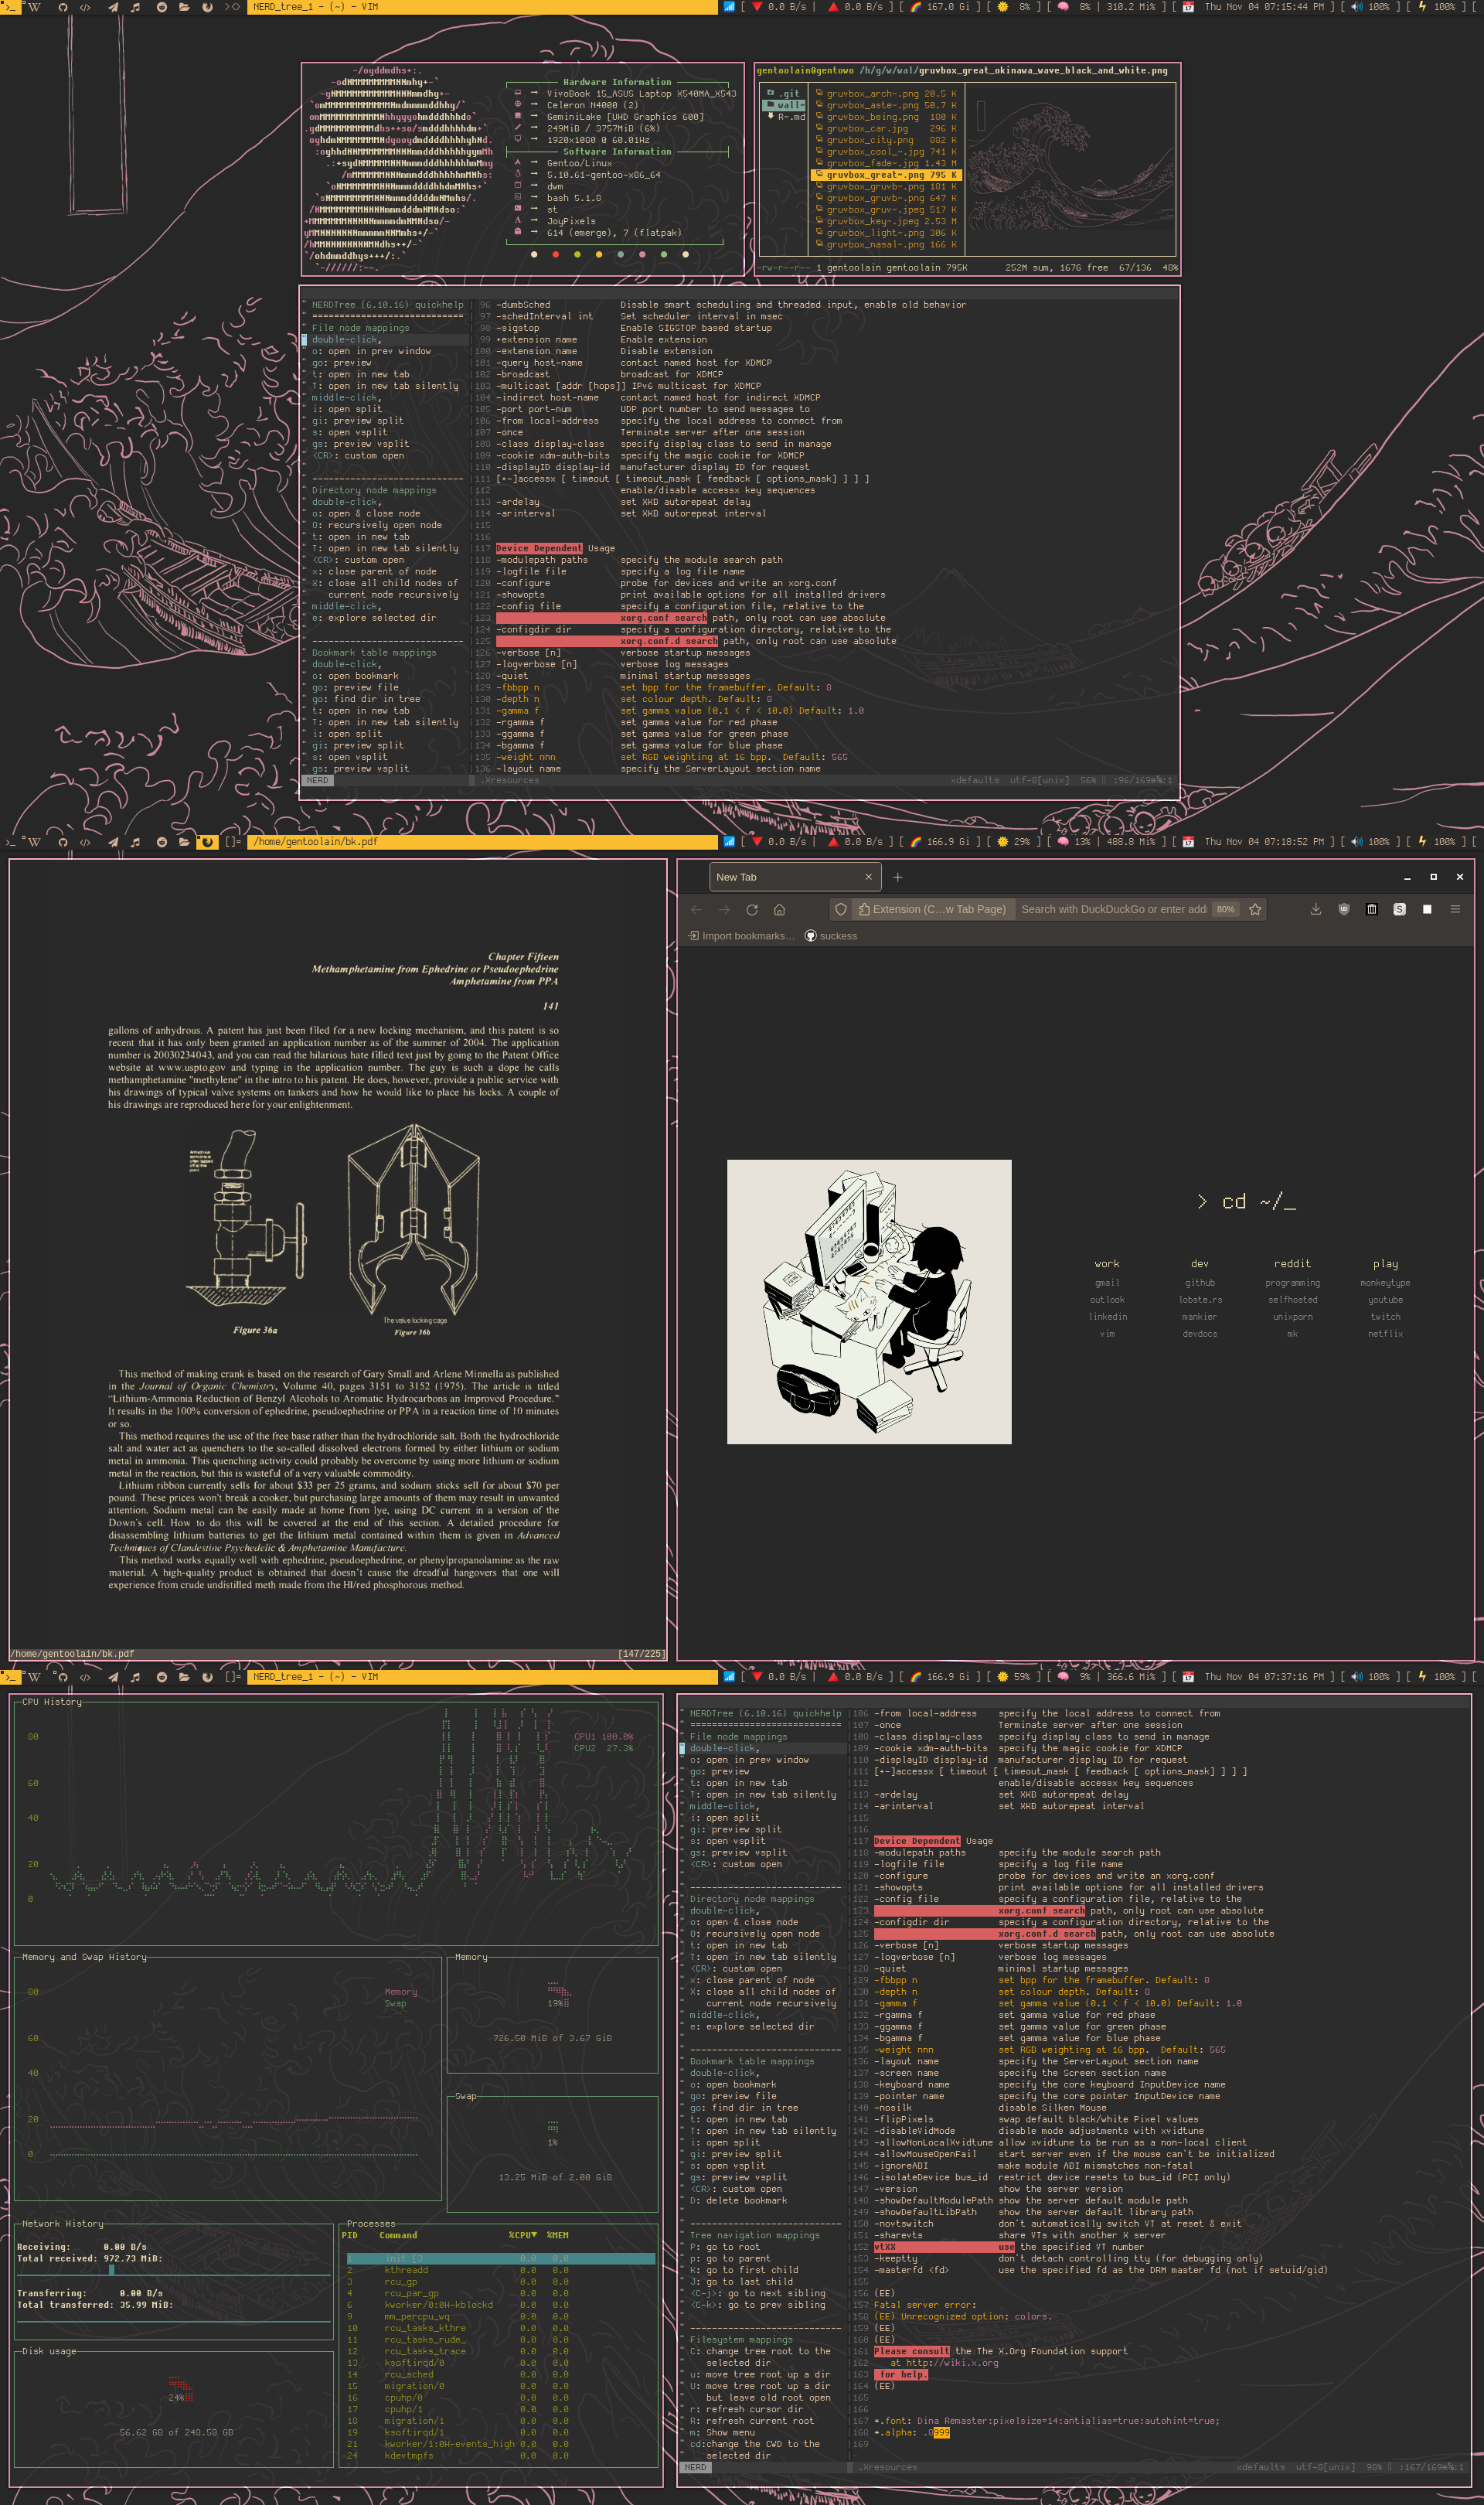
\includegraphics[scale=0.2]{Images/Rice/img1.png}
\\~\\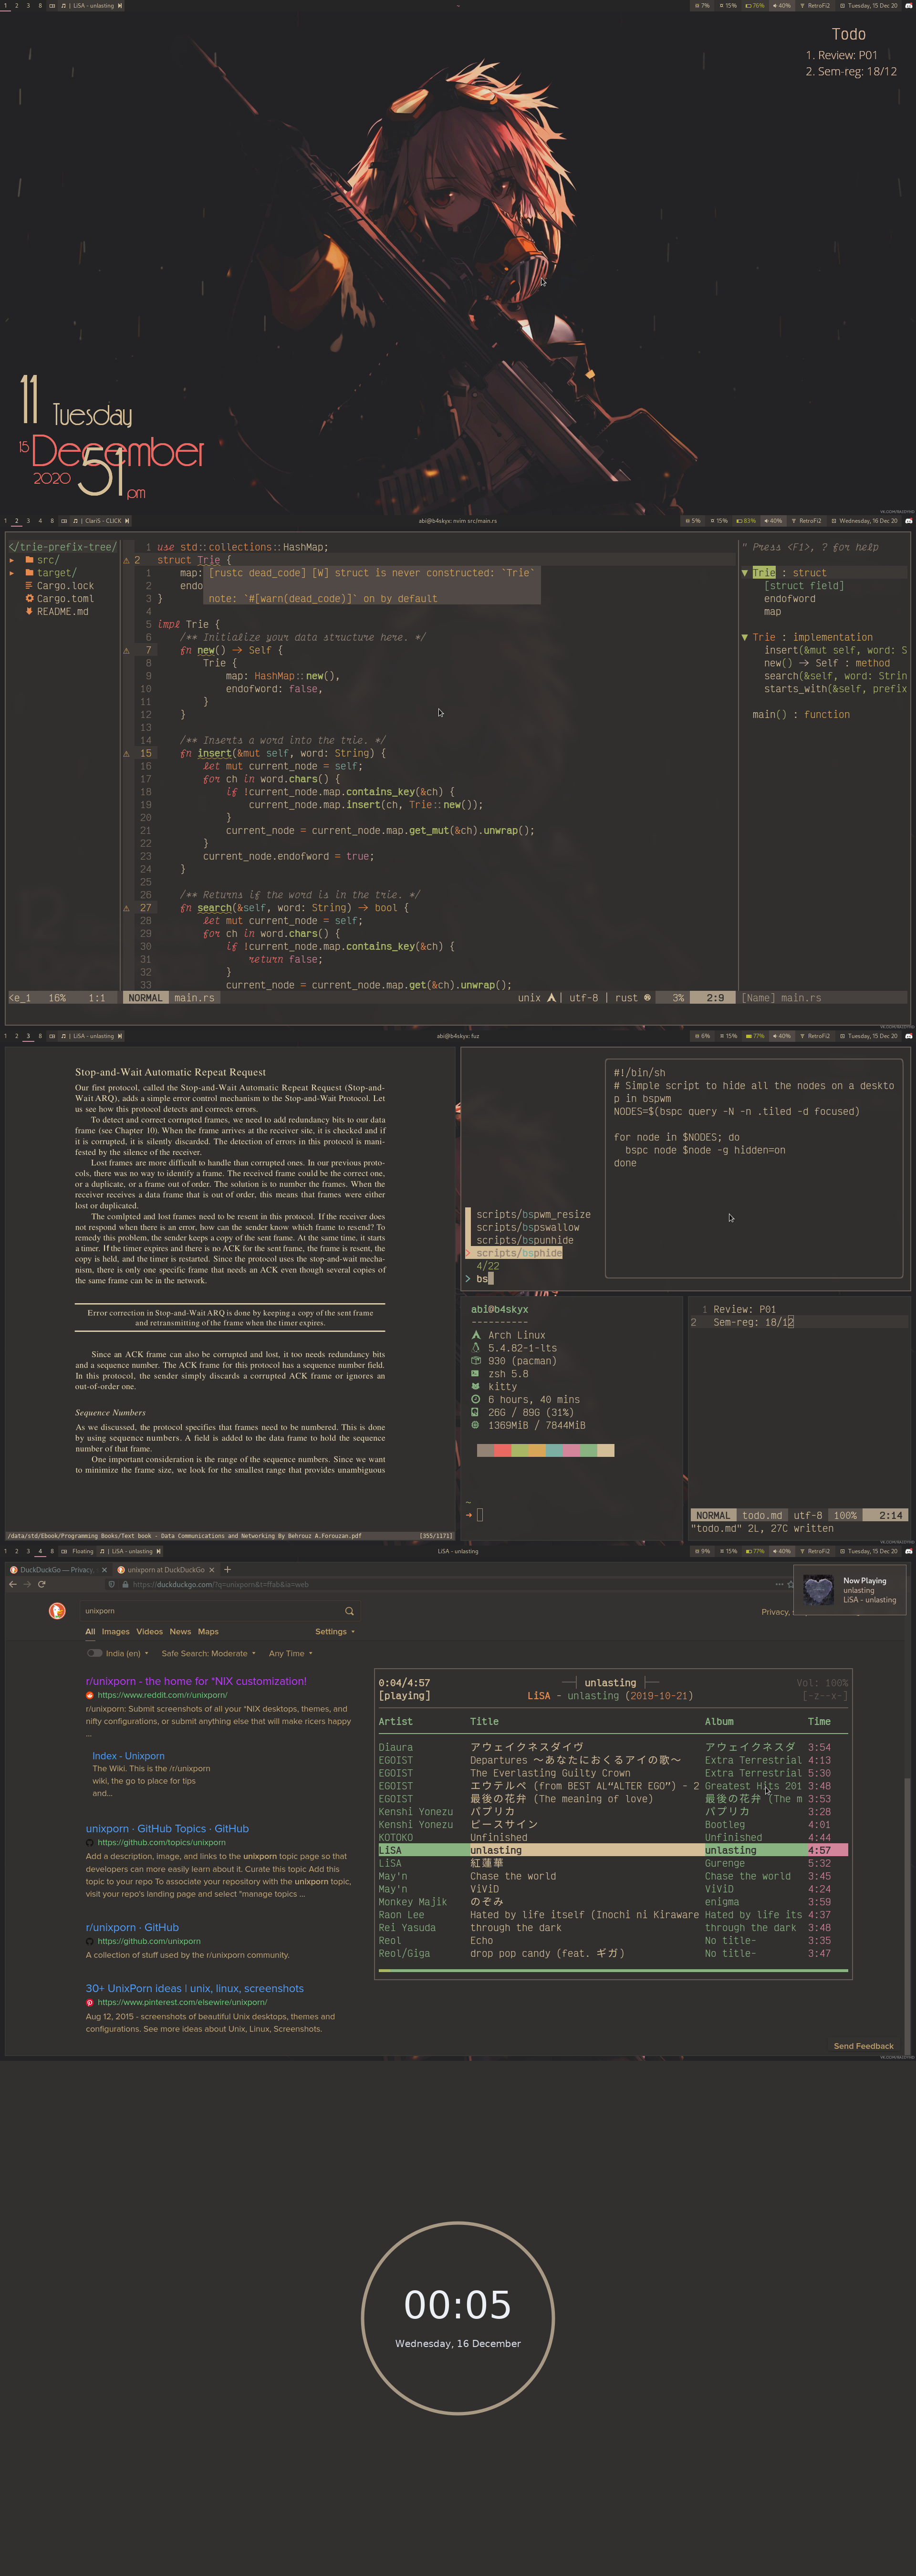
\includegraphics[scale=0.14]{Images/Rice/img2.png}
\\~\\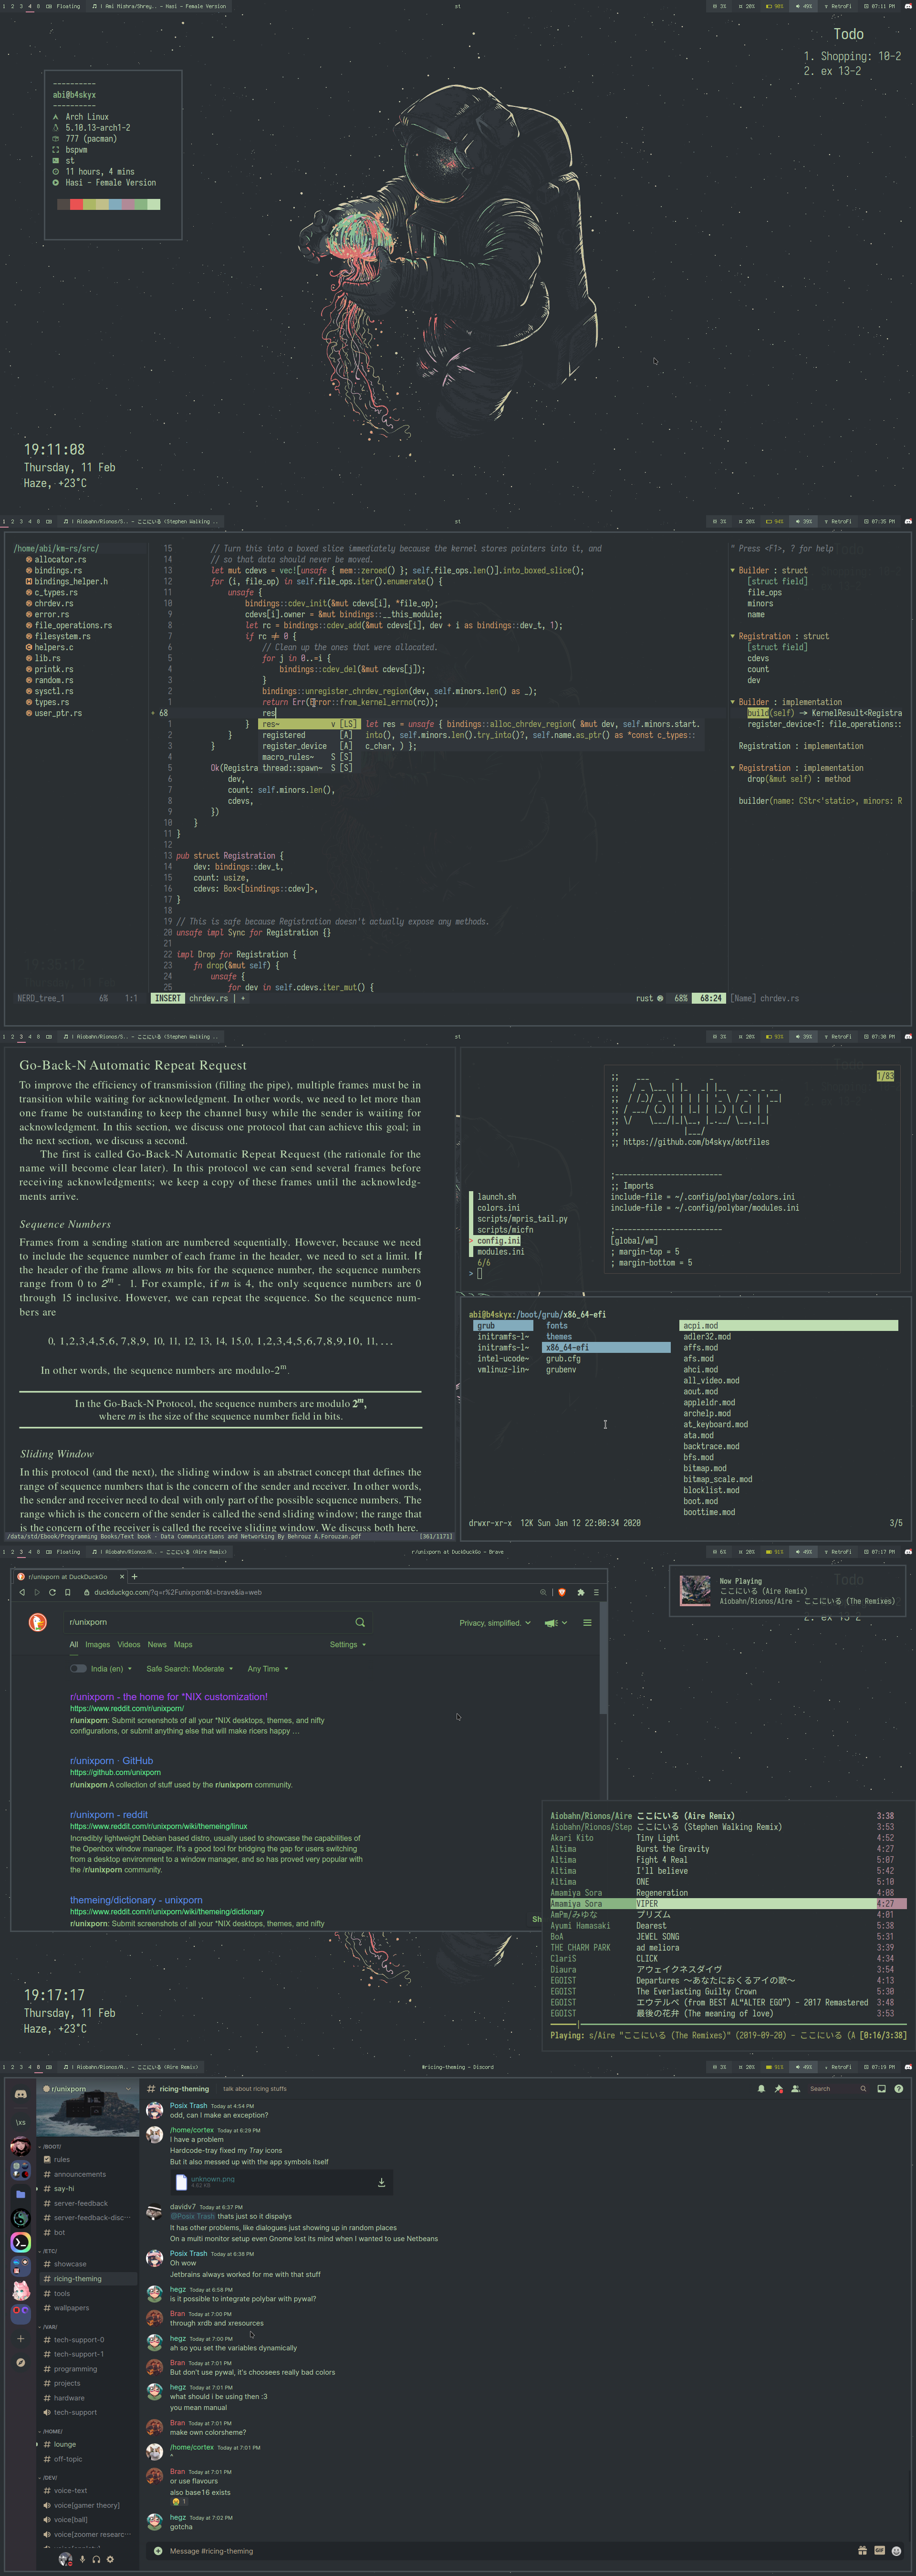
\includegraphics[scale=0.14]{Images/Rice/img3.png}
\\~\\\includegraphics[scale=0.2]{Images/Rice/img4.png}
\\~\\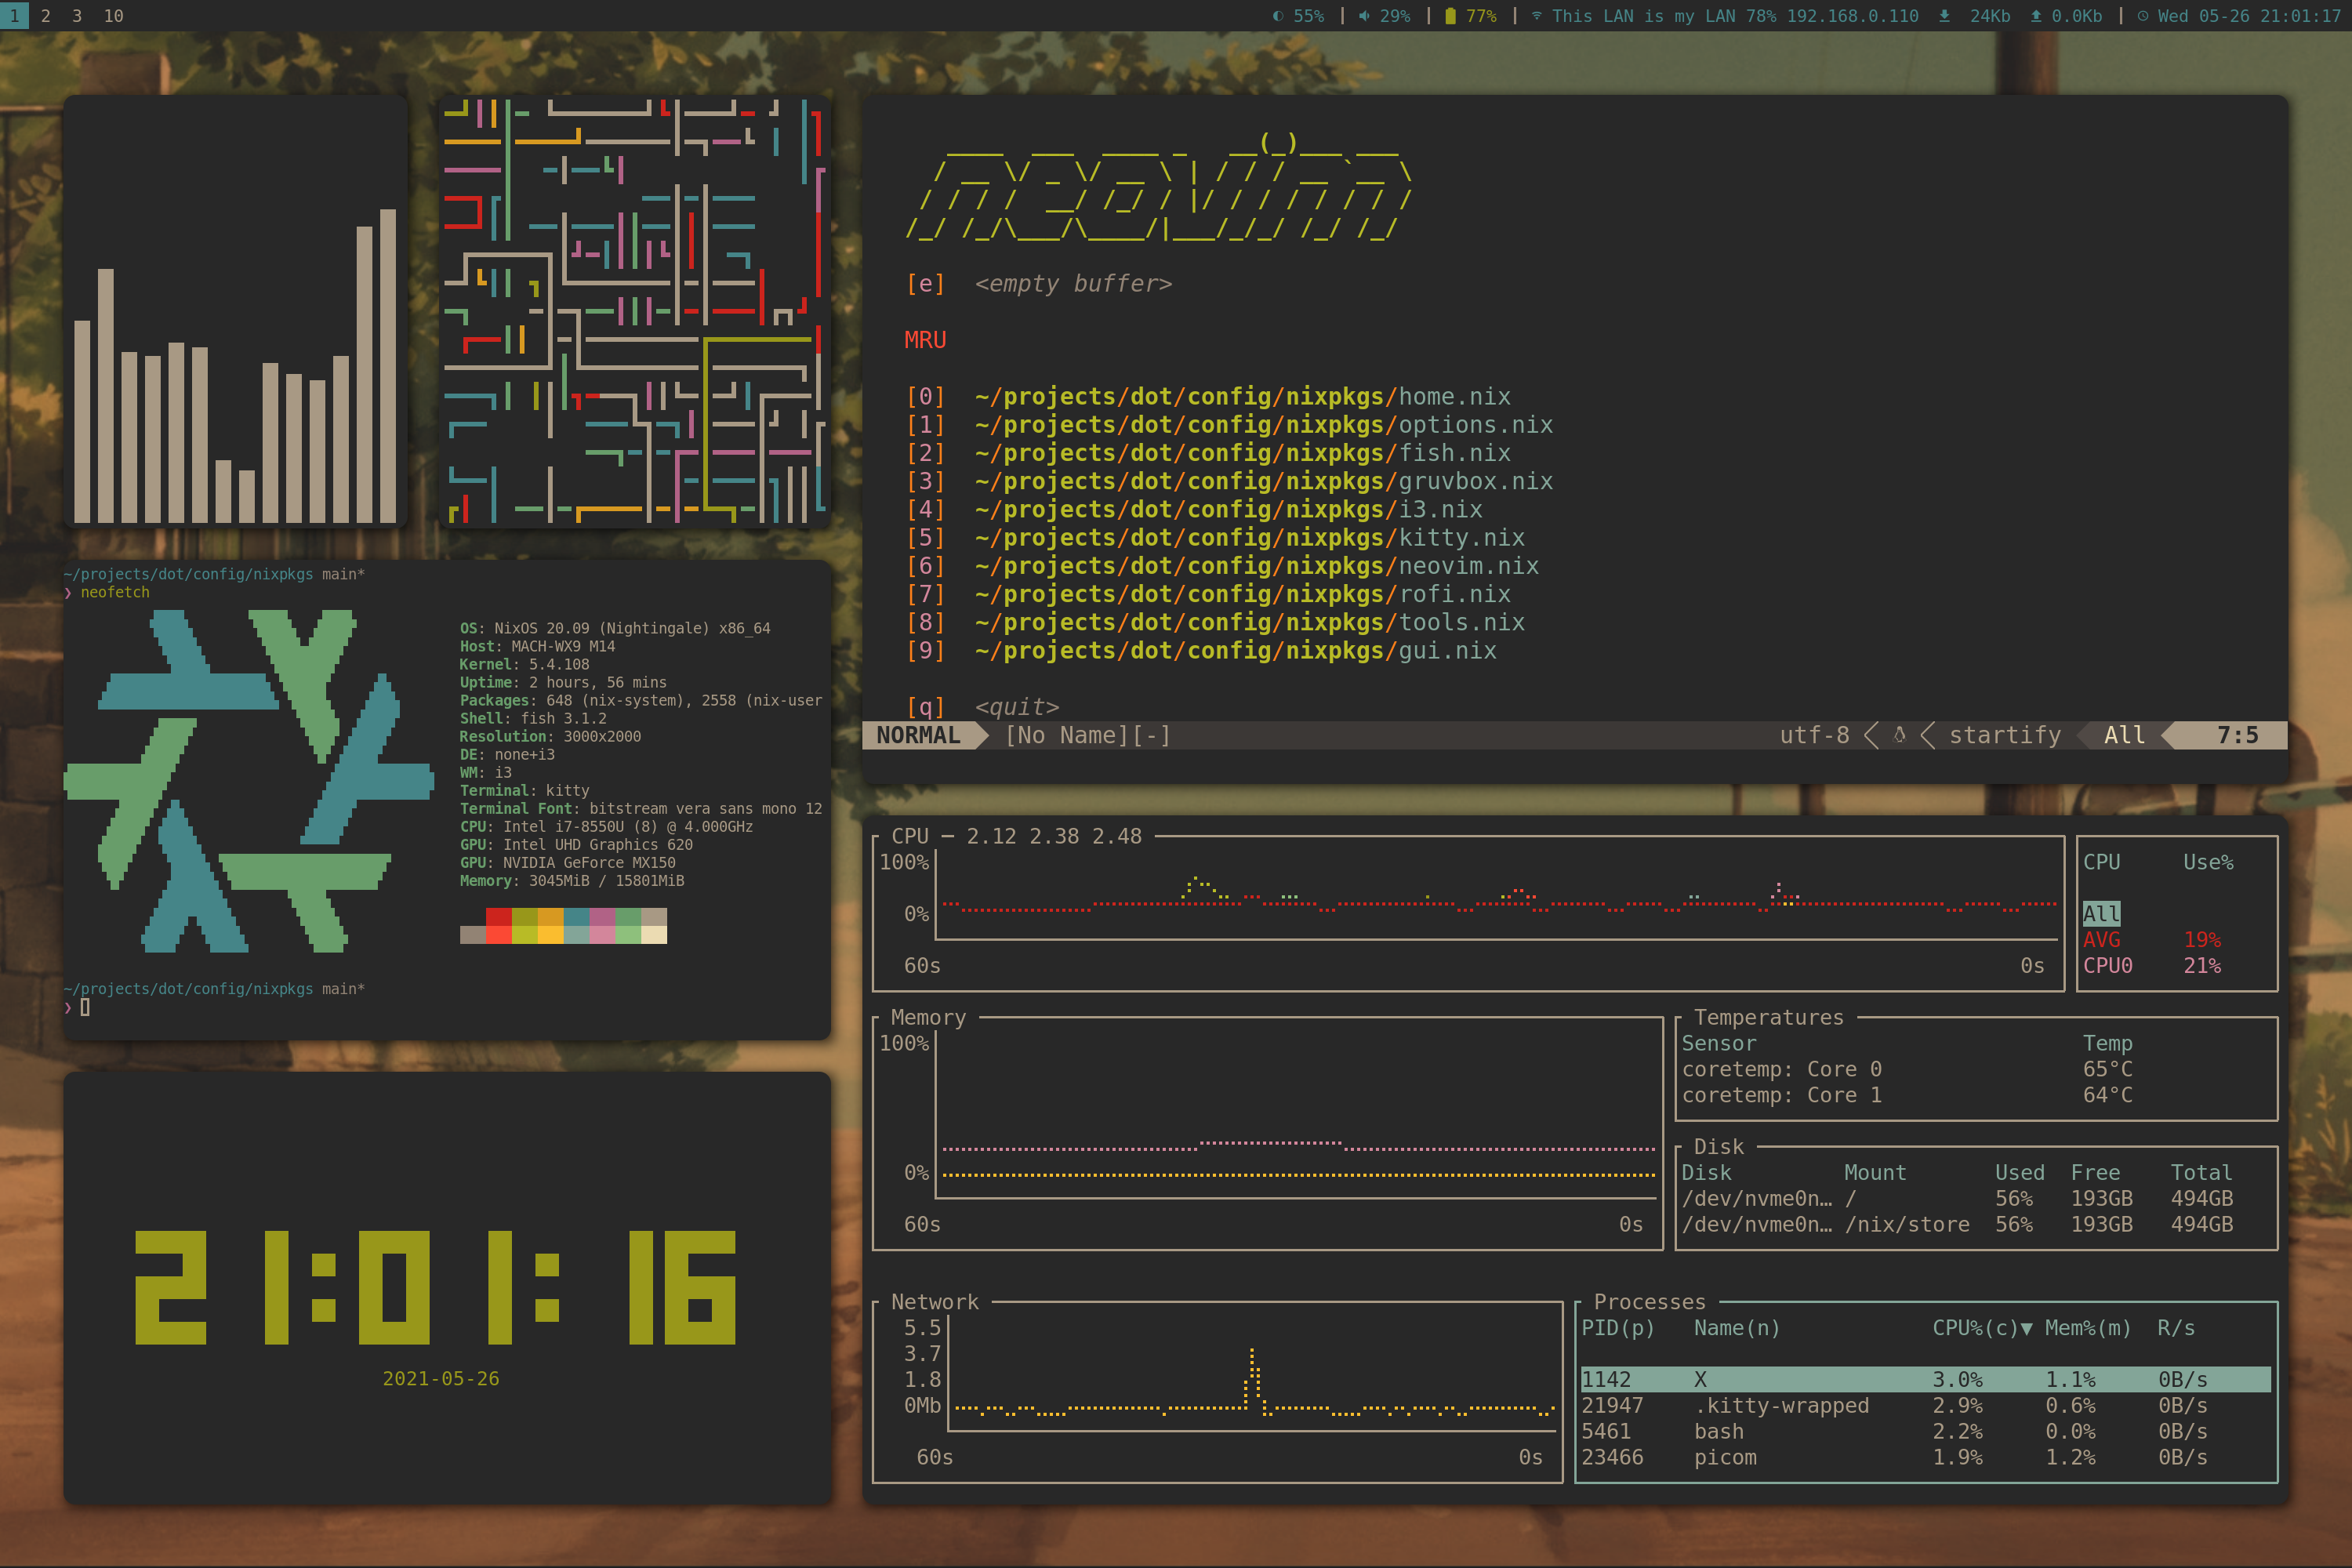
\includegraphics[scale=0.13]{Images/Rice/img5.png}





\begin{comment}
TODO :The automatic installation does not cover all the way till the base arch linux install
Summary of the keybindings are not done
Not all of the user specific scripts have been fully explained
The screen brightness light breaks, and is not really valid, maybe use xrandr?
The rice isn't that good to be honest.

THIS DOCUMENT IS NOT MEANT TO DETAIL THE SPECIFIC PROGRAMS. IT IS ONLY TO DETAIL HOW THEY CAN BE USED WITH RESPECT TO ONE ANOTHER, THE SPECIFIC IMPLEMENTATIONS CAN BE READ SEPARATELY AND NOT DISCUSSED HERE.

\end{comment}





\end{center}
\end{document}
